\usepackage[authoryear,round]{natbib}
\usepackage{multirow}

\newcommand{\sheetnum}{%
	11
}
%\setcounter{section}{\sheetnum-3}
\newcommand{\tutorialtitle}{%
    Multi-class SVM  \&
    Support Vector Regression (SVR)
}
\newcommand{\tutorialtitleshort}{%
	SVR
}
% for slides
\subtitle{\sheetnum \tutorialtitle}

%\maxdeadcycles=1000 % Workaround for ! Output loop---100 consecutive dead cycles because of too many figures

% The following use of algroithms does not work well with the notes:
%
%
%
%
% instead use the following for your algorithms:
%
%\begin{figure}[!t]
%\removelatexerror
%\begin{algorithm}[H]
    % your algo here
    %\label{alg:algolabel}
    %\caption{algocaption}
%\end{algorithm}
%\end{figure}
%\begin{algorithm}
% Below is the definition for the command \removelatexerror:
\makeatletter
\newcommand{\removelatexerror}{\let\@latex@error\@gobble}
\makeatother

\begin{document} %%%%%%%%%%%%%%%%%%%%%%%%%%%%%%%%%%%%%%%%%%%%%%%%%%%%%%%

\sheet{\sheetnum}{\tutorialtitleshort}

\ttopic{\tutorialtitle}

\columnratio{0.2,0.8}\textbf{}
\begin{paracol}{2}
%\setlength{\columnseprule}{0.1pt}
%\setlength{\columnsep}{5em}

\begin{rightcolumn}

% notes version will ignore it
\begin{frame}
\titlepage
\end{frame}

\begin{frame}
\tableofcontents
\end{frame}

\mode<all>
\section{Multi-class SVM}

\mode<presentation>{
\begin{frame} 
    \begin{center} \huge
        \secname
    \end{center}
    \begin{center}
    A very brief overview   
    \end{center}
\end{frame}
}

\begin{frame}\frametitle{The binary classification setting}

\mode<article>{
\underline{The binary classification setting}:\\
}

Classification problems have labels with only finitely many possible values.

Example: Binary classification, $y_{T} \in \{-1,1\}$:

\begin{figure}[ht]
     \centering
     \savebox{\imagebox}{
	 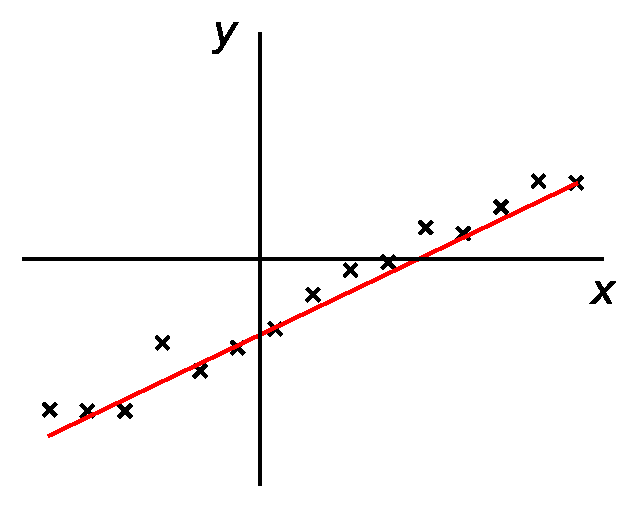
\includegraphics[width=0.35\textwidth]{img/classification_1d_sign}}%
     \begin{subfigure}[t]{0.35\textwidth}
         \centering
         \usebox{\imagebox}% Place largest image
         \caption{1D input}
         \label{fig:classification1d}
     \end{subfigure}
     \hspace{10mm}
     \begin{subfigure}[t]{0.35\textwidth}
         \centering
         \raisebox{\dimexpr.5\ht\imagebox-.5\height}{% Raise smaller image into place
         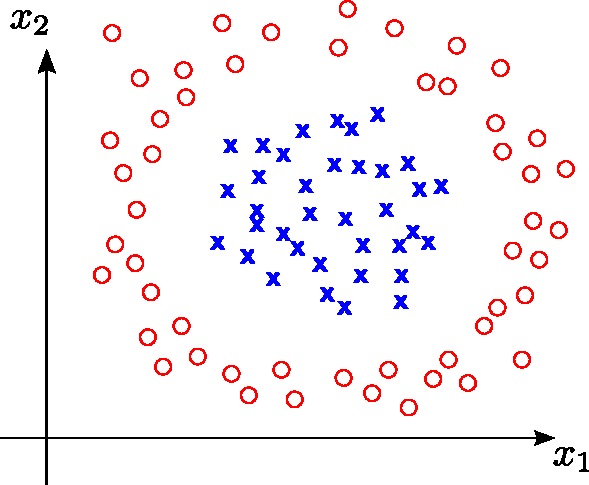
\includegraphics[width=0.99\textwidth]{img/circular}
         }
         \caption{2D input}
         \label{fig:classification2d}
     \end{subfigure}
     \caption{binary classification}
	 \label{fig:classification}
\end{figure}

\end{frame}

\begin{frame}\frametitle{The multi-class classification setting}

A set of $K>2$ classes: $\{c_{1},c_{2},\ldots,c_{K}\}$

\begin{figure}[h]
     \centering
	 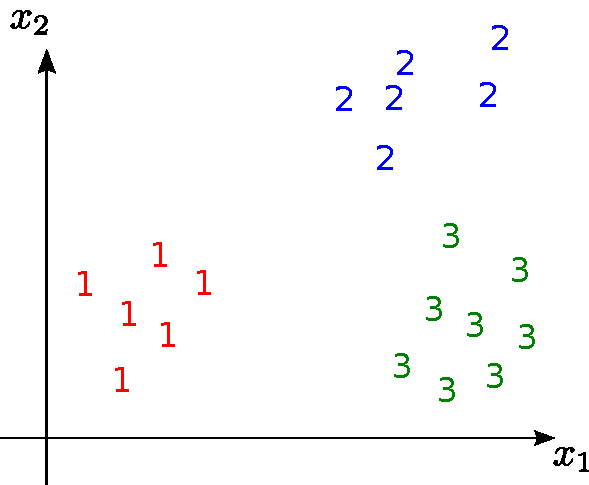
\includegraphics[width=0.35\textwidth]{img/3classes}
     \caption{multi-class classification}
	 \label{fig:multiclassification}
\end{figure}

Remains an open issue for SVMs.

\end{frame}

\subsection{One-vs-rest (one-vs-all)}

\begin{frame}\frametitle{\subsecname}

\only<1,2>{
\begin{itemize}
\item[] for each class $c_{k}$ in $\{c_{1},c_{2},\ldots,c_{K}\}$\\
do
\begin{itemize}
\item[] train a binary classifier with $c_{k}$ as its \textbf{positive} class
\item[] \textbf{all} remaining $K-1$ classes are treated collectively as the \textbf{negative} class.\\
\end{itemize}
end
\end{itemize}

\slidesonly{
\only<1>{\textbf{see blackboard}}
}

}
\only<2,3>{
%\slidesonly{
	%\begin{textblock}{}(10,5)
%}
\begin{figure}[h]
     \centering
	 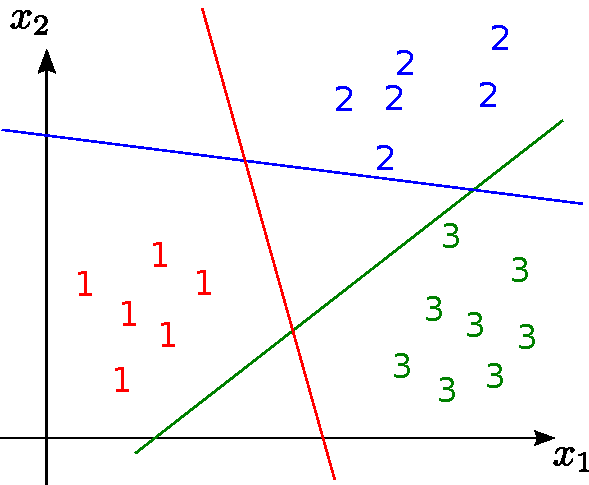
\includegraphics[width=4cm]{img/3classes_onevsall}
     \caption{$K$ one-vs-all classifiers}
	 \label{fig:multiclassification}
\end{figure}
%\slidesonly{
	%\end{textblock}
%}

\slidesonly{\vspace{-5mm}}

\question{Any potential problems with training $K$ one-vs-all classifiers?}
}

\only<3>{
\slidesonly{\vspace{-5mm}}

\begin{itemize}
\item ambiguous regions
\item needs heuristic to disambiguate (e.g. $\argmax_{k} y_{k}(\vec x)$)\\
    but any heuristic needs to deal with the different scales of each $y_{k}(\vec x)$
\item each classifier faces an imbalanced training set. In the case of SVMs, this leads to asymmetric margins. 
But ``class weighted'' SVMs exist.

\end{itemize}
}

    
\end{frame}

\begin{frame}

\begin{figure}[h]
     \centering
	 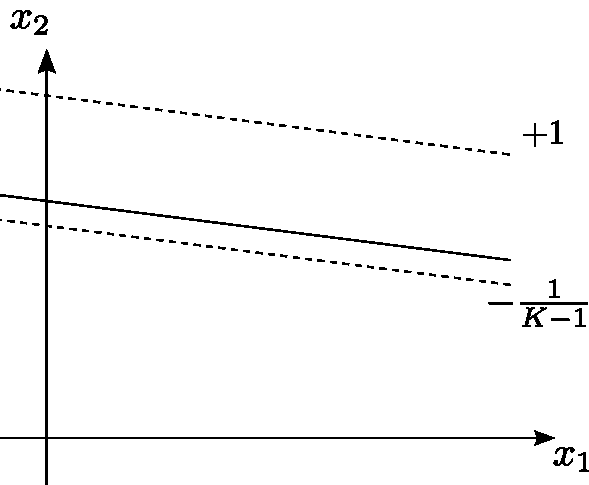
\includegraphics[width=4cm]{img/asymmetric}
     \caption{Asymmetric margins due to class imbalance}
	 \label{fig:imbalance}
\end{figure}

Actually: one-vs-rest classification for SVMs is good enough for many problems.

    
\end{frame}

\subsection{One-vs-one (all pairs)}

\begin{frame}\frametitle{\subsecname}

\# binary classifiers = $\frac{K(K-1)}{2}$ 

\begin{itemize}
\item[:-(] long test times.\\
    Testing speed can be improved by organizing the pair classifiers into a DAG\footnote{Directed Acyclic Graph, a tree would qualify.} to reduce to a subset of $K-1$ only.
\item[:-)] Training is fast as each only requires a very small subset of the data. 
\item[:-(] We still have ambiguous regions:    
\end{itemize}

\begin{figure}[h]
     \centering
	 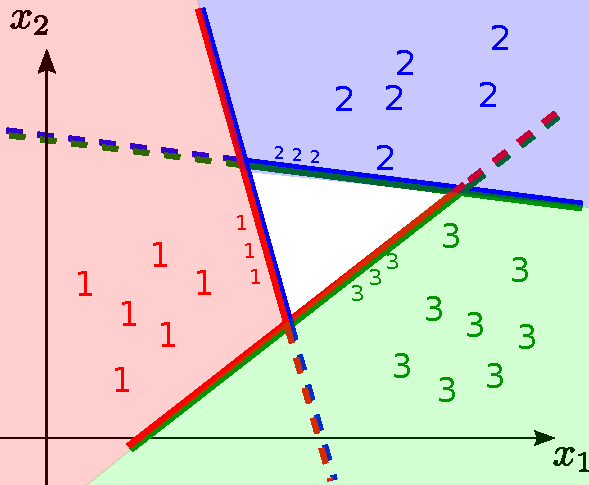
\includegraphics[width=5cm]{img/3classes_onevsone_majority}
	 \mode<article>{
     \caption{One-vs-one classification}
     }
	 \label{fig:onevsone}
\end{figure}
    
\end{frame}

\subsection{Extend with error-correcting outputs}

\begin{frame}

A rough outline of this ensemble method:

\begin{enumerate}
\item Express each class using an $L$-bit binary vector (e.g. $\{+1,-1\}$). Choose $L>K$.
\item Concatenate all vectors into a $K \times L$ matrix. 
\item Train a binary classifier to target the value of the $i$-th column in this matrix.
    \begin{itemize}
    \item If class $k$ is associated with a ``$+1$'' at the $i$-th column. All data from this class will be used as \textbf{positive} examples when training the $i$-th classifier.
    \item If class $k$ is associated with a ``$-1$'' at the $i$-th column. All data from this class will be used as \textbf{negative} examples when training the $i$-th classifier.
    \end{itemize}
\end{enumerate}
    
\end{frame}

\begin{frame}\frametitle{Example for error correcting codes}

% Please add the following required packages to your document preamble:
% \usepackage{graphicx}
\begin{table}[]
%\resizebox{\textwidth}{!}
{%
\begin{tabular}{|c|c|c|c|c|c|c|}
\hline
Class & $l_1$ & $l_2$ & $l_3$ & $l_4$ & $l_5$ & $l_6$ \\ \hline\hline
$c_{1}$ & 1 & -1 & 1 & -1 & -1 & 1 \\ \hline
$c_{2}$ & 1 & 1 & -1 & -1 & 1 & -1 \\ \hline
$c_{3}$ & -1 & 1 & -1 & 1 & -1 & 1 \\ \hline
$c_{4}$ & -1 & -1 & 1 & -1 & 1 & 1 \\ \hline
\end{tabular}%
}
\caption{Example for error correcting codes using 6-bits for 4 classes}
\end{table}

Classifier $y_{2}(\vec x)$ will use all points from $c_{2}$, $c_{3}$ as positive examples and $c_{1}$, $c_{4}$ as negative examples.

By looking at the predictions of all classifiers. One would match the $6$-bit prediction pattern with those of the 4 classes to determine which class was detected.

\end{frame}

\mode*

\mode<all>
\section{Support Vector Regression (SVR)}

\mode<presentation>{
\begin{frame} 
    \begin{center} \huge
        \secname
    \end{center}
    \begin{center}
    SVMs for regression problems   
    \end{center}
\end{frame}
}

\begin{frame}\frametitle{The classification setting}

\mode<article>{
The classification setting:\\
}

Classification problems have labels with only finite many possible values.

Example: Binary classification, $y_{T} \in \{-1,1\}$:

\begin{figure}[ht]
     \centering
     \savebox{\imagebox}{
	 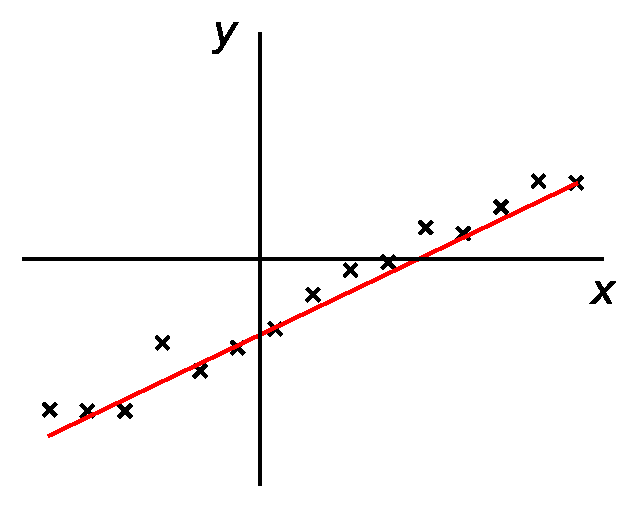
\includegraphics[width=0.35\textwidth]{img/classification_1d_sign}}%
     \begin{subfigure}[t]{0.35\textwidth}
         \centering
         \usebox{\imagebox}% Place largest image
         \caption{1D input}
         \label{fig:classification1d}
     \end{subfigure}
     \hspace{10mm}
     \begin{subfigure}[t]{0.35\textwidth}
         \centering
         \raisebox{\dimexpr.5\ht\imagebox-.5\height}{% Raise smaller image into place
         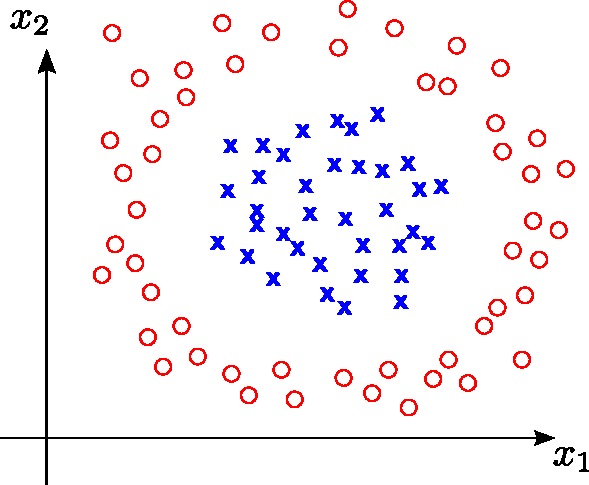
\includegraphics[width=0.99\textwidth]{img/circular}
         }
         \caption{2D input}
         \label{fig:classification2d}
     \end{subfigure}
     \caption{binary classification}
	 \label{fig:classification}
\end{figure}

\end{frame}

\begin{frame}\frametitle{Regression setting}

\mode<article>{
\underline{The Setting}:
}

\begin{itemize}
\item[] \underline{Data}:\\
    \begin{equation}
    \big\{ (\vec x^{(\alpha)}, y_{T}^{(\alpha)}\big\}_{\alpha=1}^{p}
    \end{equation}
    with $\vec x \in \R^{N}$ and $y_{T} \in \R${}

\item[] \underline{Model}:\\
    linear neuron:
    \begin{equation}
        y(\vec x; \vec w, b) = \vec w^{\top} \vec x + b
    \end{equation}


    
\end{itemize}


\begin{figure}[h]
     \centering
     \savebox{\imagebox}{
	 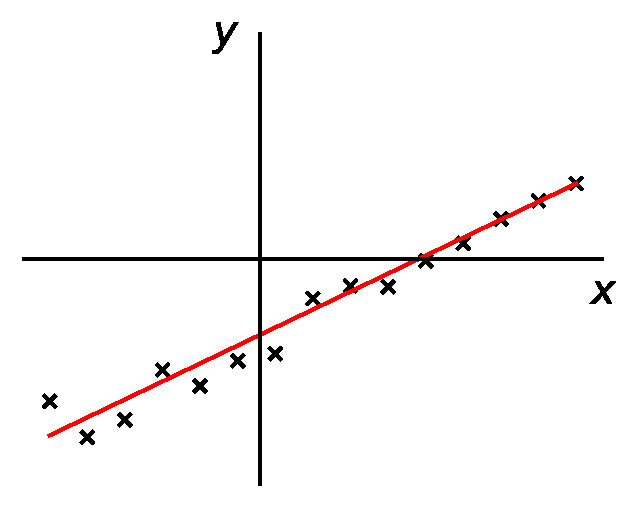
\includegraphics[width=0.35\textwidth]{img/regression_1d_linear}}%
     \begin{subfigure}[t]{0.35\textwidth}
         \centering
         \usebox{\imagebox}% Place largest image
         \caption{linear regression}
         \label{fig:regression1dlinear}
     \end{subfigure}
     \hspace{10mm}
     \begin{subfigure}[t]{0.35\textwidth}
         \centering
         \raisebox{\dimexpr.5\ht\imagebox-.5\height}{% Raise smaller image into place
         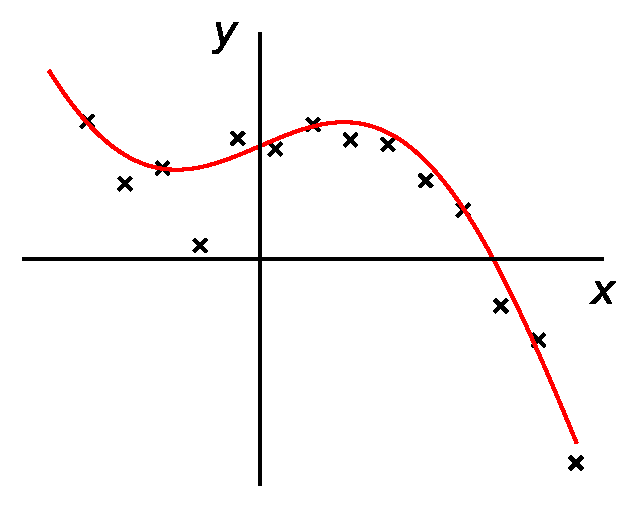
\includegraphics[width=0.99\textwidth]{img/regression_1d_nonlinear}
         }
         \caption{non-linear regression}
         \label{fig:regression1dnonlinear}
     \end{subfigure}
     \caption{scalar regression with 1D input}
	 \label{fig:regression}
\end{figure}



\end{frame}

\subsection{The $\varepsilon$-sensitive cost function for regression}

\begin{frame}\frametitle{\subsecname}

\begin{equation}
e(y(\vec x^{(\alpha)}; \vec w, b), y_{T})
= e(\underbrace{y(\vec x^{(\alpha)})}_{\substack{\text{for brevity}}}, y_{T})
= \max(~0~, \big|~y(\vec x^{(\alpha)}) - y_{T}^{(\alpha)}~\big| - \varepsilon~)
\end{equation}

\begin{itemize}
\item The cost function is parameterized by $\varepsilon${}
\item for model output
\begin{equation}
y(\vec x) \in \lbrack y_{T}-\varepsilon, y_{T}+\varepsilon\rbrack    
\end{equation}    
$\Rightarrow$ no error.
\item outside this range $\Rightarrow$ linear error
\end{itemize}

\begin{figure}[h]
     \centering
	 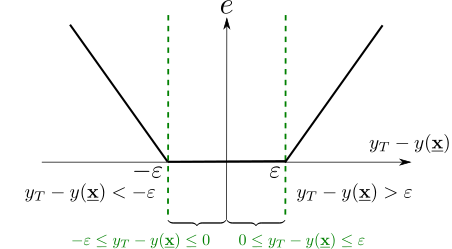
\includegraphics[width=0.7\textwidth]{img/cost_eps}%
     \caption{The cost function}
	 \label{fig:cost}
\end{figure}
    
\end{frame}

\subsubsection{Deriving the primal problem for $\varepsilon$-SVR}

\begin{frame}\frametitle{\subsubsecname}

\begin{itemize}
\item[(i)]
Simplify assumptions (will be relaxed later)
\begin{enumerate}
    \item perfect regression solution, i.e. zero error $\varepsilon$-sensitive cost,
    \item the regression problem

        \begin{equation}
        \begin{array}{ll}
        \min_{\vec w, b} & \frac{1}{2} \lVert \vec w \rVert_{2}^{2}\\
        \text{subject to} & 
        y(\vec x^{(\alpha)}) - y_{T}^{(\alpha)} \le \varepsilon\\
        &
        y_{T}^{(\alpha)} - y(\vec x^{(\alpha)}) \le \varepsilon \quad \text{for }\alpha=1,\ldots,p
        \end{array}
        \end{equation}  
        
        This is equivalent to:\\

        \begin{equation}
        \begin{array}{ll}
        \min_{\vec w, b} & \frac{1}{2} \lVert \vec w \rVert_{2}^{2}\\
        \text{subject to} & 
        \vec w^{\top} \vec x^{(\alpha)} + b - y_{T}^{(\alpha)} \le \varepsilon\\
        &
        y_{T}^{(\alpha)} - \vec w^{\top} \vec x^{(\alpha)} - b \le \varepsilon \quad \text{for }\alpha=1,\ldots,p
        \end{array}
        \end{equation}  
        
        \begin{figure}[h]
     \centering
	 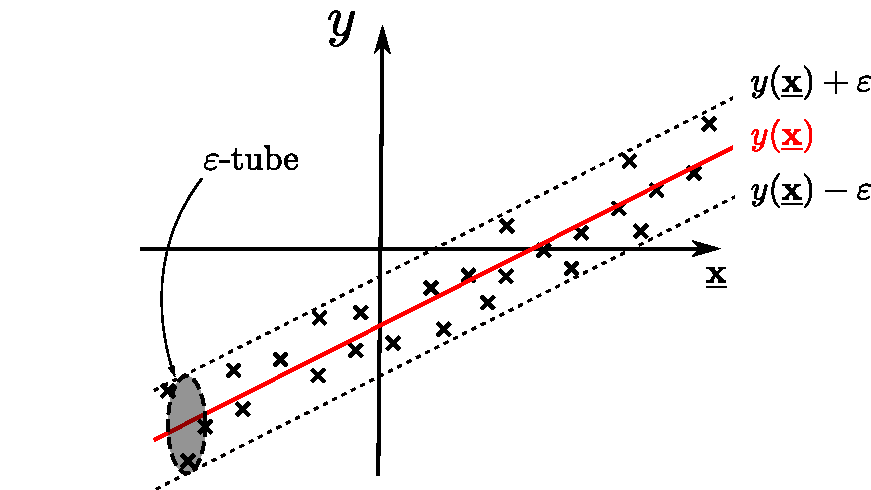
\includegraphics[width=0.7\textwidth]{img/regression_1d_linear_margin}%
     \caption{Linear model (no points outside the margin)}
	 \label{fig:model_margin}
\end{figure}


\end{enumerate}
\end{itemize}
    
\end{frame}

\mode*

\clearpage

\mode<all>
\section{$\nu$-SVR}

\mode<presentation>{
\begin{frame} 
    \begin{center} \huge
        \secname
    \end{center}
    \begin{center}   
    Essentially $\varepsilon$-SVR but treat $\varepsilon$ as a primal variable instead of a hyperparameter.
    \end{center}
\end{frame}
}

\subsection{Motivation}

\begin{frame}\frametitle{\subsecname~for $\nu$-SVR}

\mode<presentation>{

\begin{figure}[h]
     \centering
     \savebox{\imagebox}{
	 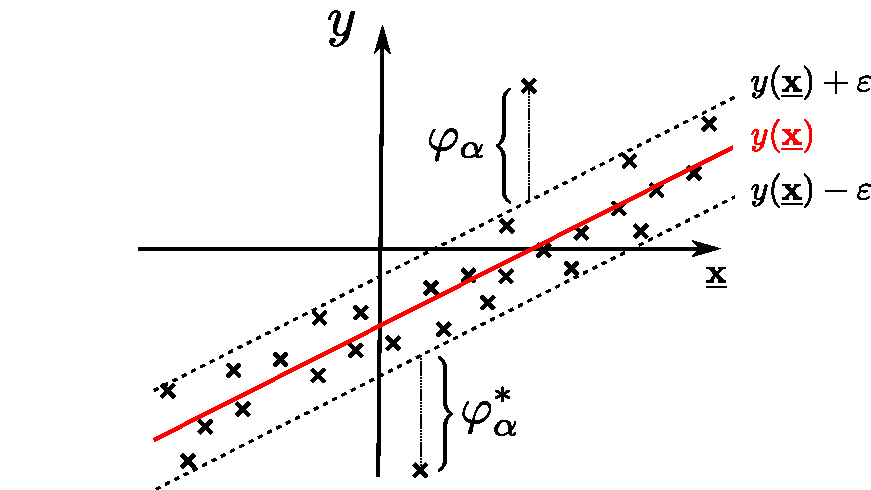
\includegraphics[width=0.4\textwidth]{img/regression_1d_linear_margin_phi}}%
     \begin{subfigure}[t]{0.4\textwidth}
         \centering
         \usebox{\imagebox}% Place largest image
     \end{subfigure}
     %\hspace{2mm}
     \begin{subfigure}[t]{0.4\textwidth}
         \centering
         \raisebox{\dimexpr.5\ht\imagebox-.5\height}{% Raise smaller image into place
         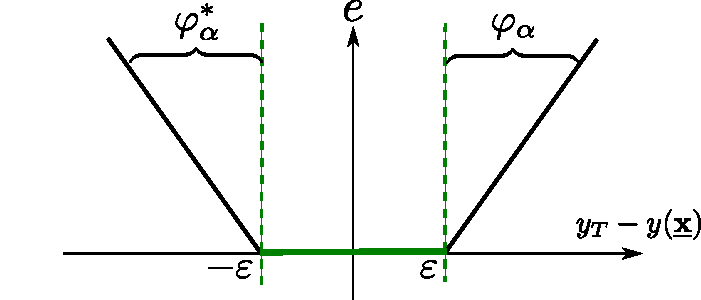
\includegraphics[width=0.99\textwidth]{img/cost_eps_phi}
         }
     \end{subfigure}
\end{figure}
}

\notesonly{
Choosing $\varepsilon$ for $\varepsilon$-SVR can be difficult as it depends on the noise in the data and this noise is unknown.
}$\varepsilon$-SVR requires treating $\varepsilon$ as a hyperparameter.
\notesonly{We therefore resort to methods such as corss-validation for choosing one value for $\varepsilon$ over another.}

$\nu$-SVR extends $\varepsilon$-SVR, by allowing the width of the ``$\varepsilon$-tube'' to adapt to the data. This is done by turning $\varepsilon$ into a \emph{primal variable}. We can then optimize w.r.t. $\varepsilon$ as we do with $\vec w, b$ and \notesonly{the set of slack variables }$\{\varphi_\alpha\}, \{\varphi_\alpha^*\}$.

\end{frame}

\subsection{Deriving the primal problem for $\nu$-SVR}

\definecolor{darkgreen}{rgb}{0,0.6,0}
\begin{frame}\frametitle{\subsecname}

\slidesonly{\vspace{-4mm}}

\begin{block}{}
     \begin{equation}
        \begin{array}{ll}
        \min_{\vec w, b,\{\varphi_\alpha\}, \{\varphi_\alpha^*\}\only<2->{, {\color{darkgreen}{\varepsilon}}}} & \frac{1}{2} \lVert \vec w \rVert_{2}^{2} + C \only<2->{\big\lbrack \nu{\color{darkgreen}\varepsilon} + } \frac{1}{p} \sum_{\alpha}^p (\varphi_\alpha + \varphi_\alpha^*) \only<2>{\big\rbrack}\\
        \text{subject to} & 
        \vec w^{\top} \vec x^{(\alpha)} + b - y_{T}^{(\alpha)} \le \varepsilon + \varphi_\alpha\\
        &
        y_{T}^{(\alpha)} - \vec w^{\top} \vec x^{(\alpha)} - b \le \varepsilon^* + \varphi_\alpha^*\\
        &\varphi_\alpha, \varphi_\alpha^* \ge 0  \qquad\qquad\qquad\qquad\quad \text{for }\alpha=1,\ldots,p \\
        &\only<2->{{\color{darkgreen}\varepsilon~\ge~0}}
        \end{array}
        \label{eq:primalnu}
     \end{equation}
     
     \slidesonly{\vspace{-3mm}}
        with $C>0$ ($C$ penalizes model error)\only<2->{, $\nu \ge 0$}
\end{block}

\pause

      \notesonly{
$\nu$-SVR extends $\varepsilon$-SVR with: 1 $\times$ new variable, 1 $\times$ new hyper-parameter, 1 $\times$ new constraint.
}

     \slidesonly{\vspace{-3mm}}

     \question{Aren't we just exchanging one hyperparameter for another? How is this better?}\\
     
\pause

     - Increased resolution of how we balance model error and model complexity. We will see that $\nu$ acts as a
     \begin{itemize}
     \item upper bound on the fraction of errors\notesonly{: $\nu \ge \frac{1}{p} \sum_{\alpha}^p (\varphi_\alpha + \varphi_\alpha^*)$}\notesonly{\\ and as a \\}
     
     \item lower bound on the fraction of SVs\notesonly{: $\nu \le \frac{\# SV}{p}$}.
     \end{itemize}
     \notesonly{The solution of the primal problem for $\nu$-SVR will enable us to discuss this in more detail (cf. \sectionref{sec:intuitionnu}}
\end{frame}


\subsection{Deriving the Lagrangian for the primal problem of $\nu$-SVR}

\subsubsection{Idenitfying the Lagrange multipliers}

\begin{frame}\frametitle{\subsecname\\ \subsubsecname}

\slidesonly{\vspace{-3mm}}

\question{Where are multipliers needed?}\\

\slidesonly{\vspace{-3mm}}

\begin{block}{The primal problem}
     \begin{equation}
        \begin{array}{lrll}
        \min_{\vec w, b,\{\varphi_\alpha\}, \{\varphi_\alpha^*\}{, {{\varepsilon}}}} && \frac{1}{2} \lVert \vec w \rVert_{2}^{2} + C {\big\lbrack \nu{\varepsilon} + } \frac{1}{p} \sum_{\alpha}^p (\varphi_\alpha + \varphi_\alpha^*) {\big\rbrack}			&\\
        \text{subject to}
        &&\vec w^{\top} \vec x^{(\alpha)} + b - y_{T}^{(\alpha)} \le \varepsilon + \varphi_\alpha		&\visible<2>{\leadsto\{\lambda_{\alpha}\}}\\
        &&y_{T}^{(\alpha)} - \vec w^{\top} \vec x^{(\alpha)} - b \le \varepsilon^* + \varphi_\alpha^*	&\visible<2>{\leadsto\{\lambda_{\alpha}^*\}}\\
        &&\varphi_\alpha \ge 0  												&\visible<2>{\leadsto\{\eta_{\alpha}\}}\\
        &&\varphi_\alpha^* \ge 0 \qquad\qquad \text{for }\alpha=1,\ldots,p 		&\visible<2>{\leadsto\{\eta_{\alpha}^*\}}\\
        &&\varepsilon \ge 0														&\visible<2>{\leadsto\delta}
        \end{array}
        %\label{eq:primalnu}
     \end{equation}
        
        with $C>0$ and $\nu \ge 0$.
\end{block}

\pause

Next: re-arrange the constraints to be in the form $f_\alpha \le 0$ to form the Lagrangian of the primal problem.

\end{frame}

\subsubsection{Re-arranging the constraints}

\begin{frame}\frametitle{\subsecname\\ \subsubsecname}

\slidesonly{\vspace{-5mm}}
\visible<1>{
Next: re-arrange the constraints to be in the form $f_\alpha \le 0$\notesonly{ to form the Lagrangian of the primal problem}:
}
\slidesonly{\vspace{-3mm}}

\mode<presentation>{
\only<1>{
\begin{block}{The primal problem}
     \begin{equation}
        \begin{array}{lrll}
        \min_{\vec w, b,\{\varphi_\alpha\}, \{\varphi_\alpha^*\}{, {{\varepsilon}}}} && \frac{1}{2} \lVert \vec w \rVert_{2}^{2} + C {\big\lbrack \nu{\varepsilon} + } \frac{1}{p} \sum_{\alpha}^p (\varphi_\alpha + \varphi_\alpha^*) {\big\rbrack}			&\\
        \text{subject to}
        &&\vec w^{\top} \vec x^{(\alpha)} + b - y_{T}^{(\alpha)} \le \varepsilon + \varphi_\alpha		&\leadsto\{\lambda_{\alpha}\}\\
        &&y_{T}^{(\alpha)} - \vec w^{\top} \vec x^{(\alpha)} - b \le \varepsilon^* + \varphi_\alpha^*	&\leadsto\{\lambda_{\alpha}^*\}\\
        &&\varphi_\alpha \ge 0  												&\leadsto\{\eta_{\alpha}\}\\
        &&\varphi_\alpha^* \ge 0 \qquad\qquad \text{for }\alpha=1,\ldots,p 		&\leadsto\{\eta_{\alpha}^*\}\\
        &&\varepsilon \ge 0														&\leadsto\delta
        \end{array}
        %\label{eq:primalnu}
     \end{equation}
        
        with $C>0$ and $\nu \ge 0$.
\end{block}
}
}
\mode<presentation>{
\only<2>{
\begin{block}{The primal problem with constraints in the form of $f_\alpha \le 0$}
     \begin{equation}
        \begin{array}{lrll}
        \min_{\vec w, b,\{\varphi_\alpha\}, \{\varphi_\alpha^*\}{, {{\varepsilon}}}} && \frac{1}{2} \lVert \vec w \rVert_{2}^{2} + C {\big\lbrack \nu{\varepsilon} + } \frac{1}{p} \sum_{\alpha}^p (\varphi_\alpha + \varphi_\alpha^*) {\big\rbrack}			&\\
        \text{subject to}
        &&\vec w^{\top} \vec x^{(\alpha)} + b - y_{T}^{(\alpha)} - \varepsilon - \varphi_\alpha	\le 0	&\leadsto\{\lambda_{\alpha}\}\\
        &&y_{T}^{(\alpha)} - \vec w^{\top} \vec x^{(\alpha)} - b - \varepsilon^* - \varphi_\alpha^*	\le 0 &\leadsto\{\lambda_{\alpha}^*\}\\
        &&- \varphi_\alpha \le 0  												&\leadsto\{\eta_{\alpha}\}\\
        && - \varphi_\alpha^* \le 0 \qquad\qquad \text{for }\alpha=1,\ldots,p 		&\leadsto\{\eta_{\alpha}^*\}\\
        && - \varepsilon \le 0														&\leadsto\delta
        \end{array}
        %\label{eq:primalnu}
     \end{equation}
        
        with $C>0$ and $\nu \ge 0$.
\end{block}
}
}

\only<3>{
\begin{block}{The primal problem with constraints in the form of $f_\alpha \le 0$}
     \begin{equation}
        \begin{array}{lrll}
        \min_{\vec w, b,\{\varphi_\alpha\}, \{\varphi_\alpha^*\}{, {{\varepsilon}}}} && \frac{1}{2} \lVert \vec w \rVert_{2}^{2} + C {\big\lbrack \nu{\varepsilon} + } \frac{1}{p} \sum_{\alpha}^p (\varphi_\alpha + \varphi_\alpha^*) {\big\rbrack}			&\\
        \text{subject to}
        &-&\{ \varphi_{\alpha} +\varepsilon+y_T^{(\alpha)} -\vec{w}^\top\vec{x}^{(\alpha)}-b \}	\le 0	&\leadsto\{\lambda_{\alpha}\}\\
        &-&\{ \varphi_{\alpha}^* 
				+\varepsilon-y_T^{(\alpha)}+\vec{w}^\top\vec{x}^{(\alpha)}+b \}	\le 0 &\leadsto\{\lambda_{\alpha}^*\}\\
        &-&\varphi_\alpha \le 0  												&\leadsto\{\eta_{\alpha}\}\\
        &-&\varphi_\alpha^* \le 0 \qquad\qquad \text{for }\alpha=1,\ldots,p 		&\leadsto\{\eta_{\alpha}^*\}\\
        &-&\varepsilon \le 0														&\leadsto\delta
        \end{array}
        %\label{eq:primalnu}
     \end{equation}
        
        with $C>0$ and $\nu \ge 0$.
\end{block}
}

\end{frame}

\begin{frame}\frametitle{\subsecname}

\slidesonly{\vspace{-5mm}}

\begin{equation}
\left.\begin{aligned}
				L(\underbrace{\vec{w},b,\{\varphi_{\alpha}\},\{\varphi_{\alpha}^*\},\varepsilon}_{\text{primal variables}},
				\underbrace{\{\lambda_{\alpha}\}, \{\lambda_{\alpha}^*\},\{\eta_{\alpha}\},\{\eta_{\alpha}^*\},\delta}_{\mathclap{\text{dual variables (Lagrange multipliers)}}})\\
				= \smallfrac{1}{2} \lVert\vec{w}\rVert^2_2+C \Big\lbrack \nu \varepsilon 
					+ \smallfrac{1}{p} \sum_{\alpha=1}^p(\varphi_{\alpha}
					+\varphi_{\alpha}^*) \Big\rbrack \\
				-\sum_{\alpha=1}^p \lambda_{\alpha} \{\varphi_{\alpha}
				+\varepsilon+y_T^{(\alpha)}
				-\vec{w}^\top\vec{x}^{(\alpha)}-b \}  \\
				-\sum_{\alpha=1}^p \lambda_{\alpha}^* \{\varphi_{\alpha}^* 
				+\varepsilon-y_T^{(\alpha)}+\vec{w}^\top\vec{x}^{(\alpha)}+b \} \\ 
				-\sum_{\alpha=1}^p \eta_{\alpha} \varphi_{\alpha} 
				- \sum_{\alpha=1}^p \eta_{\alpha}^* \varphi_{\alpha}^* 
				- \delta \varepsilon
			\end{aligned}\right.
\end{equation}

with $\{\lambda_{\alpha}\}, \{\lambda_{\alpha}^*\},\{\eta_{\alpha}\},\{\eta_{\alpha}^*\},\delta \ge 0$

\end{frame}

\subsection{Optimizing $\nu$-SVR}

\begin{frame}\frametitle{\subsecname}

\begin{enumerate}
\item We start with optimizing the Lagrangian of the \emph{primal problem}. As we did with SVMs and C-SVMs, this is achieved by
\begin{enumerate}
\item calculating the derivatives of $L$ w.r.t. \emph{primal variables} $\vec w, b, \varphi_\alpha, \varphi_\alpha^*, \varepsilon$
\item setting the partial derivatives to zero. (\textbf{see homework})
\end{enumerate}

\item Substituting the solutions to the \emph{primal problem} back into the Lagrangian yields the Lagrangian of the \emph{dual problem}\notesonly{, which can be expressed in terms of the \emph{dual variables} only}:
		\begin{equation}
		  \max_{\lambda_{\alpha}, \lambda_{\alpha}^*}
		  - \smallfrac{1}{2}\sum_{\alpha,\beta=1}^p(\lambda_{\alpha}^* -
		  \lambda_{\alpha}) (\lambda_{\beta}^* - \lambda_{\beta})
		  (\vec{x}^{(\alpha)})^\top\vec{x}^{(\beta)} +
		  \sum_{\alpha=1}^p(\lambda_{\alpha}^* 
		  - \lambda_{\alpha})y_T^{(\alpha)}
		  \nonumber
		\end{equation}
		s.t. $\forall \alpha \in \{1,\ldots,p\}$:
		$$
		  0 \leq \lambda_{\alpha} \leq \smallfrac{C}{p}
		  \,, \;\;
		  0 \leq \lambda_{\alpha}^* \leq \smallfrac{C}{p}
		  \,, \;\;
		  \sum_{\alpha=1}^p(\lambda_{\alpha} - \lambda_{\alpha}^*) = 0 
		  \,, \;\;
		  \sum_{\alpha=1}^p(\lambda_{\alpha} + \lambda_{\alpha}^*) 
		  \leq  \nu C \,.  \nonumber
		$$
\end{enumerate}


\end{frame}


\subsubsection{An intuition for $\nu$}\label{sec:intuitionnu}

\begin{frame}{Only}\frametitle{\subsubsecname}

\mode<presentation>{

     \placeimage{11}{1}{img/regression_1d_linear_margin_phi_cropped_small_err}{width=3.5cm}
}

\notesonly{
We look at the part of the primal problem in which $\nu$ and $\varepsilon$ interact\footnote{This is based on my understanding of Ch. 9.3 from \citep{scholkopf2001learning} and the paper \citep{scholkopf2000new}}:
}

\slidesonly{\vspace{-20mm}}

\begin{minipage}{7.5cm}

\begin{block}{The primal problem for $\nu$-SVR (the parts where $\nu$ and $\varepsilon$ interact)}
\slidesonly{\vspace{-5mm}}
	\begingroup
	\footnotesize
     \begin{equation}
        \begin{array}{ll}
        \min_{\vec w, b,\{\varphi_\alpha\}, \{\varphi_\alpha^*\}, \varepsilon} & \\[-1mm]
        & \kern-11ex\frac{1}{2} \lVert \vec w \rVert_{2}^{2} + C \big\lbrack {\color{blue}\nu \varepsilon} + \frac{1}{p} {\color{magenta}\sum_{\alpha}^p \overbrace{(\varphi_\alpha + \varphi_\alpha^*)}^{\text{errors}}} \big\rbrack\\[2mm]
        \text{subject to} &
        \varepsilon~\ge~0\\
        \end{array}
        \label{eq:primalnuepsonly}
     \end{equation}
     
     \slidesonly{\vspace{-2mm}}
        with $C>0$, $\nu \ge 0$, $\alpha=1,\ldots,p$
     \endgroup
\end{block}
\end{minipage}

\begin{enumerate}
\item<only@1> $\varepsilon = 0$:
\begin{itemize}
\item[$\Rightarrow$] All points are \textbf{outside} the $\varepsilon$-tube. All points are SVs, i.e. $\frac{\#\mathrm{SV}}{p}=1$.
\item[$\Rightarrow$] The \textcolor{magenta}{sum of errors} will be $> 0$
\end{itemize}
\pause
\item[]<only@2->As $\varepsilon$ increases from $0$:
\begin{itemize}
\item[$\Rightarrow$]<only@2-> \notesonly{The term }${\color{blue}\nu\varepsilon}$ \textbf{increases} proportionally to $\nu$
\item[$\Rightarrow$]<only@2,3> more points fall \textbf{inside} the $\varepsilon$-tube, \notesonly{leaving }a fraction $\frac{\#\mathrm{SV}}{p}$ of points outside the $\varepsilon$-tube \notesonly{which }are SVs\\
\item[$\Rightarrow$]<only@4-> \notesonly{The fraction decreases as $\varepsilon$ increases.} $\varepsilon \uparrow \;\;\leadsto\;\; \frac{\#\mathrm{SV}}{p} \downarrow$
 and the \textcolor{magenta}{sum of errors} \slidesonly{$\downarrow$}\notesonly{will \textbf{decrease}} proprtionally to $\frac{\#\mathrm{SV}}{p}$

\only<5,6>{ 
\question{Does $\varepsilon$ grow indefinitely?}\\
}

\only<6,7>{
\only<6>{- No, }$\varepsilon$ stops growing as soon as the \textcolor{magenta}{sum of errors} $\corresponds~\frac{\#\mathrm{SV}}{p}$ stops decreasing. But when?\\
}

\only<7->{
$\varepsilon$ stops growing as soon as $\frac{\#\mathrm{SV}}{p} \le \nu$

\question{Where does $\frac{\#\mathrm{SV}}{p} \le \nu$ come from?} 
}

\mode<article>{

- Justifying this requires part of the solution of the primal problem:
 
\begin{eqnarray}
				\frac{\partial L}{\partial \varepsilon} &=& \nu C - \smallsum{\alpha=1}{p} \lambda_\alpha
				- \smallsum{\alpha=1}{p} \lambda_\alpha^* - \delta
				\;\;\stackrel{!}{=}\;\; 0\\
				&\Rightarrow& \; \delta \;\;=\;\; \nu C - \smallsum{\alpha=1}{p} 
				(\lambda_\alpha + \lambda_\alpha^*) \\
				&\stackrel{\delta \geq 0}{\Rightarrow}&
				\nu C \;\geq\; \smallsum{\alpha=1}{p} 
				(\lambda_\alpha + \lambda_\alpha^*)
\end{eqnarray}
}

\only<7->{
\slidesonly{
 \begingroup
 \footnotesize
$$
				\frac{\partial L}{\partial \varepsilon} \stackrel{!}{=} 0\;\; \stackrel{\text{at } \varepsilon^{\mathrm{opt}}}{\Rightarrow} \;\; 
				\nu C \geq~{\color{red}\smallsum{\alpha=1}{p} 
				(\lambda_\alpha + \lambda_\alpha^*)}
				$$
\endgroup
}
}%only

\end{itemize}


\end{enumerate}


\end{frame}


\mode*

%\mode<all>
%
\subsubsection{An intuition for $\nu$}\label{sec:intuitionnu}

\mode<presentation>{
\begin{frame}\frametitle{\subsubsecname}
\mode<presentation>{

     \placeimage{11}{3.5}{img/regression_1d_linear_margin_phi_cropped_small_err}{width=3.5cm}
}

\begin{minipage}{7.5cm}

\begin{block}{The primal problem for $\nu$-SVR (the parts where $\nu$ and $\varepsilon$ interact)}
\slidesonly{\vspace{-5mm}}
	\begingroup
	\footnotesize
     \begin{equation}
        \begin{array}{ll}
        \min_{\vec w, b,\{\varphi_\alpha\}, \{\varphi_\alpha^*\}, \varepsilon} & \\[-1mm]
        & \kern-11ex\frac{1}{2} \lVert \vec w \rVert_{2}^{2} + C \big\lbrack {\color{blue}\nu \varepsilon} + \frac{1}{p} {\color{magenta}\sum_{\alpha}^p \overbrace{(\varphi_\alpha + \varphi_\alpha^*)}^{\text{errors}}} \big\rbrack\\[2mm]
        \text{subject to} &
        \varepsilon~\ge~0\\
        \end{array}
        \label{eq:primalnuepsonly}
     \end{equation}
     
     \slidesonly{\vspace{-2mm}}
        with $C>0$, $\nu \ge 0$, $\alpha=1,\ldots,p$
     \endgroup
\end{block}
\end{minipage}

\slidesonly{\vspace{10mm}}

We can try to understand the role of $\nu$ by looking at cases for $\varepsilon$:
\begin{enumerate}
\item When $\varepsilon=0$ 
\item As $\varepsilon$ \textbf{increases} from $0$, thus lowering the \textcolor{magenta}{sum of errors}
\item As $\varepsilon$ \textbf{decreases} from some large positive value, thus increasing the fraction of support vectors $\frac{\#\mathrm{SV}}{p}$
\end{enumerate}
    
\end{frame}
}

\begin{frame}%{Only}\frametitle{\subsubsecname}

\mode<presentation>{

     \placeimage{11}{1}{img/regression_1d_linear_margin_phi_cropped_small_err}{width=3.5cm}
}

\notesonly{
We look at the part of the primal problem in which $\nu$ and $\varepsilon$ interact\footnote{This is based on my understanding of Ch. 9.3 from \citep{scholkopf2001learning} and the paper \citep{scholkopf2000new}}:
}

%\slidesonly{\vspace{-20mm}}

\begin{minipage}{7.5cm}

\begin{block}{%The primal problem for $\nu$-SVR (the parts where $\nu$ and $\varepsilon$ interact)
}
\slidesonly{\vspace{-5mm}}
	\begingroup
	\footnotesize
     \begin{equation}
        \begin{array}{ll}
        \min_{\vec w, b,\{\varphi_\alpha\}, \{\varphi_\alpha^*\}, \varepsilon} & \\[-1mm]
        & \kern-11ex\frac{1}{2} \lVert \vec w \rVert_{2}^{2} + C \big\lbrack {\color{blue}\nu \varepsilon} + \frac{1}{p} {\color{magenta}\sum_{\alpha}^p \overbrace{(\varphi_\alpha + \varphi_\alpha^*)}^{\text{errors}}} \big\rbrack\\[2mm]
        \text{subject to} &
        \varepsilon~\ge~0\\
        \end{array}
        \label{eq:primalnuepsonly}
     \end{equation}
     
     \slidesonly{\vspace{-2mm}}
        with $C>0$, $\nu \ge 0$, $\alpha=1,\ldots,p$
     \endgroup
\end{block}
\end{minipage}

\begin{enumerate}
\item<only@1> $\varepsilon = 0$:
\begin{itemize}
\item[$\Rightarrow$] All points are \textbf{outside} the $\varepsilon$-tube.{}
\item[$\Rightarrow$] All points are SVs, i.e. $\frac{\#\mathrm{SV}}{p}=1$.
\item[$\Rightarrow$] The \textcolor{magenta}{sum of errors} will be $> 0$
\end{itemize}
\pause
\item<only@2-6>As $\varepsilon$ \textbf{increases} from $0$:
\begin{itemize}
\item[$\Rightarrow$]<only@3> \notesonly{The term }${\color{blue}\nu\varepsilon}$ \textbf{increases} proportionally to $\nu$
\item[$\Rightarrow$]<only@3> more points fall \textbf{inside} the $\varepsilon$-tube

\item[$\Rightarrow$]<only@3-> \notesonly{The fraction of points \textbf{outside} decreases as $\varepsilon$ increases, i.e} 
$\varepsilon \uparrow \;\;\leadsto\;\;$ \textcolor{magenta}{sum of errors} $\downarrow$

\only<3>{ 
\question{Does $\varepsilon$ grow indefinitely?}\\
}

\only<4-6>{\notesonly{{- No, }}$\varepsilon$ stops growing as soon as the \textcolor{magenta}{sum of errors} stops decreasing. But when?\\

\slidesonly{\underline{Hint}:}\notesonly{Remember from \eqref{eq:srmnu},} $\nu$-SVR \emph{optimizes} $\varepsilon$.} 

\only<5,6>{
	\begingroup
	\slidesonly{\scriptsize}
    \begin{align}
\only<5,6>{   
\frac{\partial}{\partial \varepsilon}
 \Big\lbrack 
 {\color{blue}\nu \varepsilon}& 
 + \frac{1}{p} {\color{magenta}\sum_{\alpha=1}^p (\varphi_\alpha + \varphi_\alpha^*)} 
 \Big\rbrack
 \eqexcl 0\notesonly{\\}\slidesonly{\quad}
 \Leftrightarrow \quad \frac{\partial}{\partial \varepsilon} {\color{blue}\nu \varepsilon} \notesonly{&}= -\frac{\partial}{\partial \varepsilon} 
 \Big(
 \frac{1}{p} {\color{magenta}\sum_{\alpha=1}^p (\varphi_\alpha + \varphi_\alpha^*)}
 \Big)
}
\only<6>{
 \intertext{At optimum, we have:}
 \Rightarrow \;  &-\frac{\partial}{\partial \varepsilon} 
 \Big(
 \overbrace{
 \frac{1}{p} {\color{magenta}\sum_{\alpha=1}^p (\varphi_\alpha + \varphi_\alpha^*)}
 }^{
 \text{fraction of errors}}
 \Big) \bigg|_{\varepsilon^{\mathrm{opt}}} = \nu{}
 }
\end{align}
\endgroup

\only<6>{
$\varepsilon$ grows as long as $\frac{1}{p} {\color{magenta}\sum_{\alpha=1}^p (\varphi_\alpha + \varphi_\alpha^*)} \le \nu$\\
$\nu$ is an \emph{upper bound} on the \emph{fraction of errors}.
}
}

\end{itemize}
\item<only@7-> As $\varepsilon$ \textbf{decreases}, starting from some large positive value:
\begin{itemize}
\item[$\Rightarrow$]<only@2-> \notesonly{The term }${\color{blue}\nu\varepsilon}$ \textbf{decreases} proportionally to $\nu$

\only<8->{
$\varepsilon$ decreases as long as $\frac{\#\mathrm{SV}}{p} \ge \nu$

\question{Where does $\frac{\#\mathrm{SV}}{p} \ge \nu$ come from?} 
}

\mode<article>{
%TODO FIX from here, this should lead to lower bound NOT upper bound
- Justifying this requires part of the solution of the primal problem:
 
\begin{eqnarray}
				\frac{\partial L}{\partial \varepsilon} &=& \nu C - \smallsum{\alpha=1}{p} \lambda_\alpha
				- \smallsum{\alpha=1}{p} \lambda_\alpha^* - \delta
				\;\;\stackrel{!}{=}\;\; 0\\
				&\Rightarrow& \; \delta \;\;=\;\; \nu C - \smallsum{\alpha=1}{p} 
				(\lambda_\alpha + \lambda_\alpha^*) \\
				&\stackrel{\delta \geq 0}{\Rightarrow}&
				\nu C \;\geq\; \smallsum{\alpha=1}{p} 
				(\lambda_\alpha + \lambda_\alpha^*)
\end{eqnarray}
}

\only<9->{
\slidesonly{
 \begingroup
 \footnotesize
$$
				\frac{\partial L}{\partial \varepsilon} \stackrel{!}{=} 0\;\; \stackrel{\text{at } \varepsilon^{\mathrm{opt}}}{\Rightarrow} \;\; 
				\nu C \geq~{\color{red}\smallsum{\alpha=1}{p} 
				\overbrace{(\lambda_\alpha + \lambda_\alpha^*)}^{> 0 \text{ for SVs only}}} {\propto} \frac{\#\mathrm{SV}}{p}
				$$
\endgroup
}
}%only
\item[$\Rightarrow$]<only@10> $\nu$ acts as a \emph{lower bound} on the fraction of SVs, i.e. $\nu \le \frac{\# SV}{p}$.
\end{itemize}
\end{enumerate}


\end{frame}

%\mode*

%\clearpage

\section{References}
\begin{frame}[allowframebreaks] \frametitle{References}
	\scriptsize
	\bibliographystyle{plainnat}
	\bibliography{bibliography}
\end{frame}

\end{rightcolumn}
\end{paracol}

\end{document}
